\documentclass{article}
\usepackage[utf8]{inputenc}
\usepackage{graphicx}
\usepackage{hyperref}
\usepackage{cite}
\usepackage[margin=1.4in]{geometry}
\graphicspath{ {./images/} }

\title{Agent-based models of voluntary compliance in non-pharmaceutical interventions for epidemic control}
\author{Robert Brian Milligan, Supervised by Julian Garcia Gallego \& Buser Say}
\date{7 July 2022}


\begin{document}


\maketitle

\begin{abstract}
Epidemic modelling has proven vital for understanding ways in which governments, workplaces and other decisions makers may seek to control the spread of COVID-19. Although many computational models of disease spread exist, not many consider human behaviour explicitly. In this paper, we extend a network-based agent based model to account for ways in which agents can comply or not comply with voluntary non-pharmaceutical interventions. We investigate non-strategic and strategic models of agent compliance and find that the lower the natural reproduction rate of the disease, the higher the chance of achieving success with voluntary non-pharmaceutical interventions. For high R0 values, the best results were found when compliance benefit increase is based on the number of close contacts in an individual has, Whereas for lower R0 values, the best results were found when the benefit for compliance related to looking at the number of agents one was in contact with, that was either symptomatic, hospitalised, fatality or in quarantine. In short, voluntary non-pharmaceutical interventions work best when the natural spread of the disease is relatively slow.
\end{abstract}


\newpage 

\tableofcontents

\newpage 

\section{Introduction}

Mathematical and computational models are important in designing policies to deal with pandemics. 
Standard mathematical models typically assume an infinite population and place proportions of this population into compartments ~\cite{cooper_mondal_antonopoulos_2020}. 
The traditional compartmental model is known as SIR, (Susceptible, Infectious and Recovered). 
Extensions to this basic model typically add new compartments and flows between them to account for additional elements or assumptions. 
Some common examples of variations on SIR models are SEIR, SIS and SIRV. 
SEIR, for example adds a new Exposed compartment to account for incubation periods. 
SIS models assume that once an individual recovers from the disease are not immune and re-enter the susceptible compartment.
SIRV models add a Vaccinated state whereby susceptible individuals who move to the vaccinated state cannot become infected with the disease.
When solving these models mathematically, numerical solutions can be found with standard numerical methods. \newline

When agent heterogeneity is important, as it is the case in this paper, agent based models are a popular choice. 
These models typically have a finite number of agents which interact with each other in some manner.
Moreover, these models can allow for agents to be heterogeneous not just with their personal attributes, but also with how they interact with their environment.\newline
Most epidemiological models do not incorporate behavioural elements, or if they do, they do it in simple ways such as compartmental models that incorporate "aggregate states". One such example is~\cite{karaivanov_2020}, which considers six different behavioural scenarios which would change based on the time of the simulation or having a certain threshold of positive test, positive cases or deaths per day.\newline

This paper investigates the modification of an existing model disease spread produced by Ryan McGee and used as a part of various peer reviewed research articles ~\cite{mcgee_homburger_williams_bergstrom_zhou_2021} ~\cite{mcgee_homburger_williams_bergstrom_zhou_2021_2}. 
We have looked at applying this model to the situation of COVID-19 in a childcare setting and involves creating both non strategic and strategic behavioural choice models. Specifically behaviour in this model relates to compliance to various actions the agent can choose to comply with when requested such as doing a COVID rapid antigen test whenever they have symptoms of the virus. \newline

The non strategic model gives agents a fixed cost of complying with requested actions with each individual calculating a perceived reward. This reward is based on a mix of local situations such as if they are in close contact with an agent who has a symptomatic case of the disease, and a global situation such as the percentage of the group that have reported a positive test within the last two weeks. The strategic model considers agents which know how all other agents will act and use this information to help them decide if it in their interest to comply. This incorporates a cost of compliance, a reward as well as a minimum number of agents who need to be compliant to see a reward for the group. \newline

The rest of this paper is organised as follows. Section 2 describes the basic model. Section 3 describes the base benchmark model. Section 4 introduces the non-strategic model. Section 5 introduces the various strategic models. Section 6 shows the results of running the models. Finally, section 7 discusses the results and future work.

\newpage
\section{Description of the Basic Model \label{description}}

In this section I describe the basic model, for which extensions are presented. 
This model is an Agent Based Model (ABM). 
The model was specifically designed to evaluate the effects of surveillance testing and partial vaccination for COVID-19.\newline

Agents can belong to one and only one compartment representing their state. 
When an Agent becomes infected they progress though states ending up either in the Recovered or Fatality. 
The model considers the states of Susceptible, Exposed, Pre-Infectious, Infectious-Asymptomatic, Infectious-Symptomatic, Hospitalised, Fatality and Recovered.
Agents who are Susceptible represents agents who have not yet come in to contact with the disease. 
Agents who are Exposed are those agents who have interacted with an infectious agent and have caught the disease.
Agents then move to Infectious Pre-Symptomatic. This is a stage where they can spread the disease, have no symptoms and can show up as positive if the agent takes a test. This addition was added so that agents who will develop a symptomatic case will not test before they develop symptoms but can still spread the disease.
Agents then move to either Infectious Asymptomatic or Infectious Symptomatic, the difference being is that asymptomatic cases are unaware they have the disease. Symptomatic cases may take a disease test as a result of them noticing symptoms and have the chance of moving into the hospitalised group. These two compartments were added as COVID-19 can be experienced as a Symptomatic or Asymptomatic disease. Agents who are Infectious Symptomatic can progress into Hospitalised and then potentially Fatality. Agents in either of these groups cannot spread the disease to anyone else in the network.
Agents who are Recovered represent those once infectious agents who have fully recovered and gained immunity to the disease. 
Importantly the model assumes that once an agent recovers from the disease they can no longer become infectious. \newline 
All the compartments except Hospitalised and Fatality can have agents in a mirror state where they are also isolated, meaning they cannot acquire the disease or spread it to any other agents in the network. Once an agent catches the disease they move along the stages of the disease until they are a fatality or recovered, at any point they have the ability to move across to the mirror isolation state. Agents who are in a Hospitalised, Fatality or in a Quarantined state cannot pass on the disease to anyone else in the network.


\begin{figure}[h!]
\centering
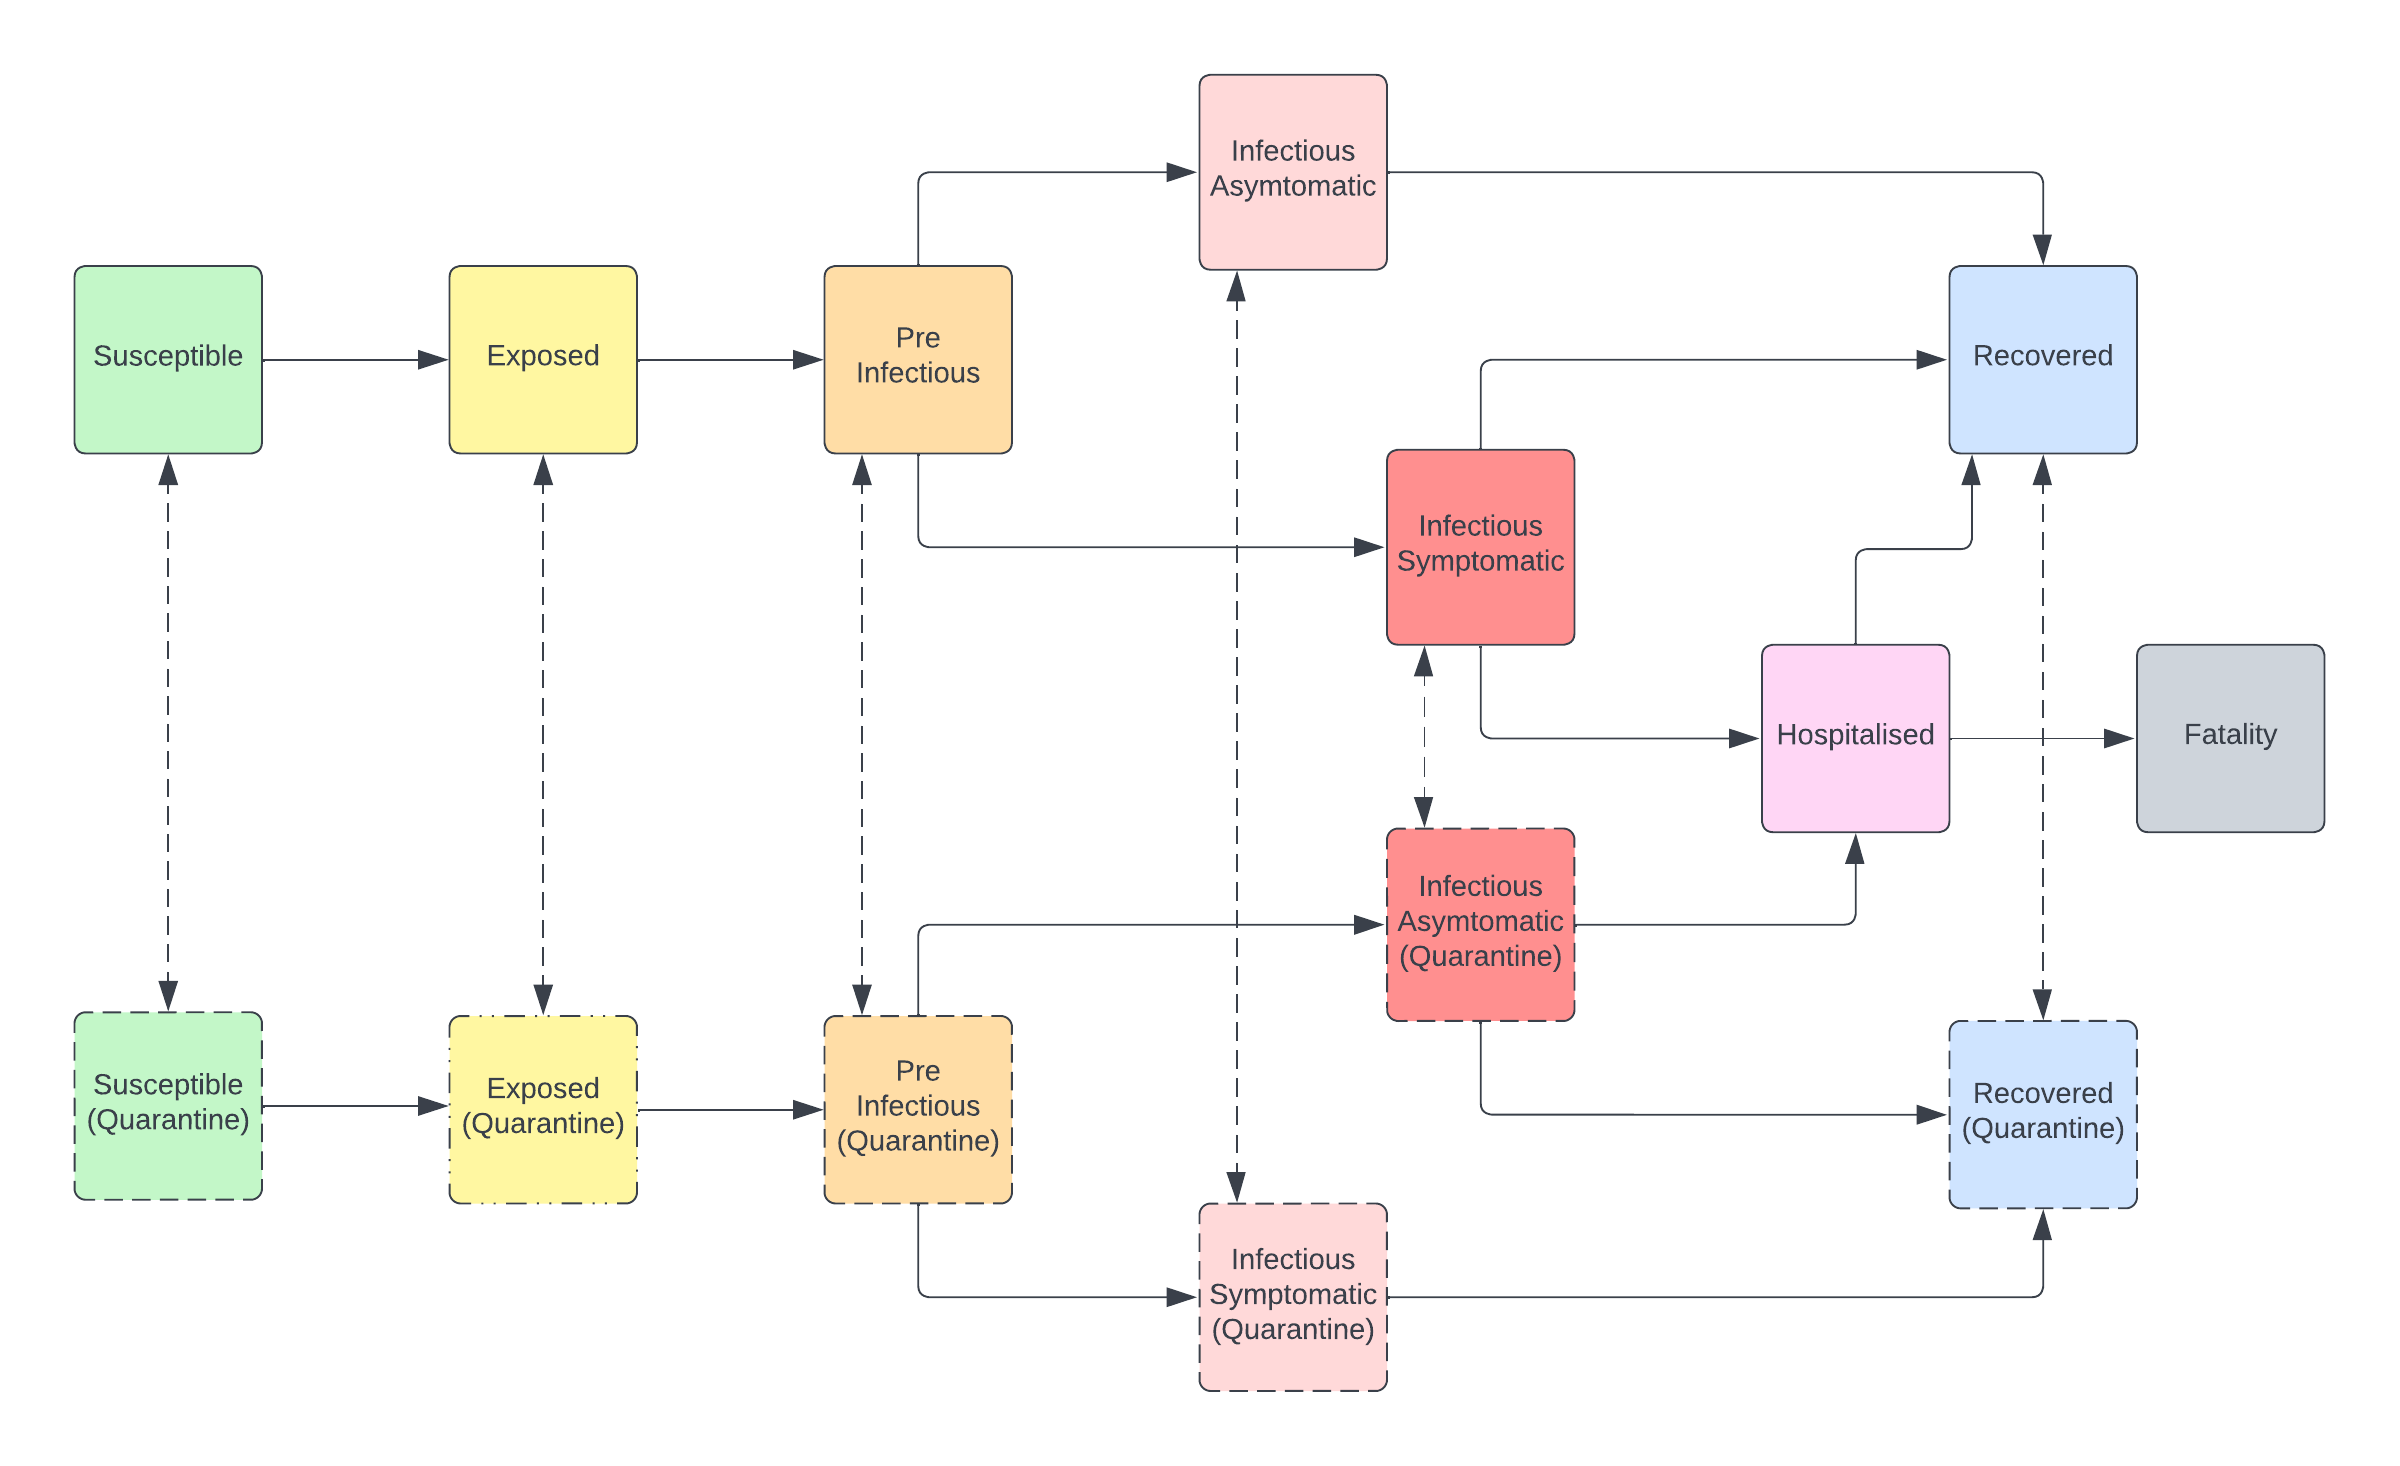
\includegraphics[width=\textwidth]{SIR}
\caption{A diagram of the existing seirplus model with its various compartments ~\cite{mcgee_2021}.The dashed arrows show those agents can move back and forth between. However. for the implemented models in this paper isolation compliance is set at 100\%, thus agents who have entered Quarantine will only ever leave Infectious Asymptomatic (Quarantine) to go to Hospitalised, or from Recovered (Quarantine) to Recovered.}
\end{figure}

\newpage


\subsection{Using networks to model contacts}

We use the version of seirsplus that uses one simple network connected network designed to simulate a workplace. These large networks are made up of a number of cohorts which are loosely connected and each of these cohorts can have a number of subgroups which are highly connected. The network is set up before the simulation begins and is randomly generated every time the simulation is run. Once the network is generated its structure does not change throughout the simulations run.  Agents are arranged in this network as its nodes and are connected by edges representing which other nodes are their close contacts. 80\% of disease spread is though the close contact edges and 20\% is spread randomly. These close contacts are the way in which we assign the agents view of their local situation.


\newpage


\subsection{Compliance}
The model uses a variety of parameters some of which relate to the compliance of actors to perform certain actions when asked. For this paper those which are relevant are those related to surveillance testing, testing if showing symptoms and quarantining if receiving back a positive test. Each day agents will be asked to do a disease test if their day has come up on a surveillance testing schedule or if they currently have a symptomatic case of the disease. However, there is a compliance value to decide if they go through with the requested action. The base model uses more than these three compliance parameters, but they are effectively removed by setting their compliance value to a negative number so that they never occur. In the existing model a parameter to set and it sets a proportion of agents to always comply and another set to never comply. This is set at the start of the simulation and never changes. In the modification of seirplus the model is changed so that this value is recalculated on every day of the simulation. This is done by setting each agent with an initial compliance value in a given range. If the benefit to compliance on that given day is greater than that initial compliance value then they become compliant. \newline

This leads to three systems of compliance which will be discussed in detail in the latter sections. The default setting where agents are given an initial value for compliance and is unchanging e.g. 50\% are set to comply and they will always do so. The non strategic model where agents are given an initial compliance and can become more compliant depending on the agents view of those other agents around them and network statistics they may have access to. The strategic model where agents utilise knowledge of the number of agents in the network who will comply to make a decision to comply or not.\newline

It should be noted the model has a few limitations. Having all agents always test on the same day, thus if semi-weekly is chosen, all agents will be asked to test on Monday and Thursday each week. the structure of the network is unchanging and has not ability for agents to join, leave or change who their close contacts are. Additionally, all values for the false negative rate for tests, fatality and hospitalisation rates are the same for all agents. This is a result of the existing model not having a system where agents can be assigned different ages in the same network and the ability to assign different false negative rate for individual or types of agents.




\newpage
\section{Benchmark Baseline Model}

We choose to create our benchmarks around COVID spread in childcare settings. 
This is an interesting case, because we focus on voluntary surveillance testing, and this is exactly how the Victorian government chose to do surveillance in childcare scenarios, by providing free antigen tests for free, but allowing the community to decide whether to test or not \footnote{See more at \url{https://www.premier.vic.gov.au/supporting-families-free-rats-school}}.  .  
In addition, this allows us to consider networks of relatively small size, which implies we do not need massive computational infrastructure to produce results. \newline 


The network structure of the model can be used to reflect the dynamics that would be apparent in a child care building and parameters could be chosen to match this specific scenario.\newline

\begin{tabular}{|c|c|}
\hline
\textbf{Parameter} & \textbf{Value} \\ \hline
Test False Negative Rate (RAT) & $0.36$ as per~\cite{van_de_mortel_2022} \\ \hline
R0 &  $9.5$ or $5.4$ as per Omicron and  \\
&  Delta variants respectively~\cite{liu_rocklov_2022} \\ \hline
Number of Survillence Tests A Week&  Two each week ~\cite{premier_of_victoria_2022} \\ \hline
Number of Agents & $100$\% \\ \hline
Number of Cohorts & $5$, typical number of rooms in  \\ 
& a childcare setting \\\hline
Mean Number of Connections Between Cohorts  & $6$ \\ \hline
Density of Edges in Cohort Networks  & $0.15$ \\ \hline
\end{tabular}
\newline


\begin{figure}[h!]
\centering
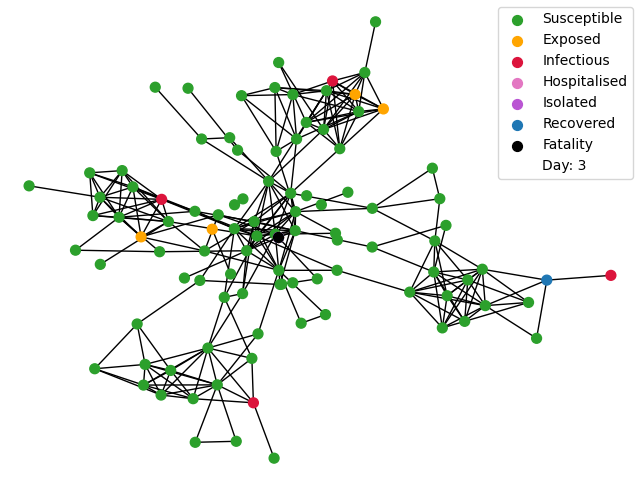
\includegraphics[width=\textwidth]{network}
\caption{An Example Network of 100 Agents. 5 distinct groups can be observed with high connectivity within the groups and low connectivity between the groups. It is also observed that three of the four exposed agents are those who are a close contact of an infectious agent}
\end{figure}

\begin{figure}
\centering
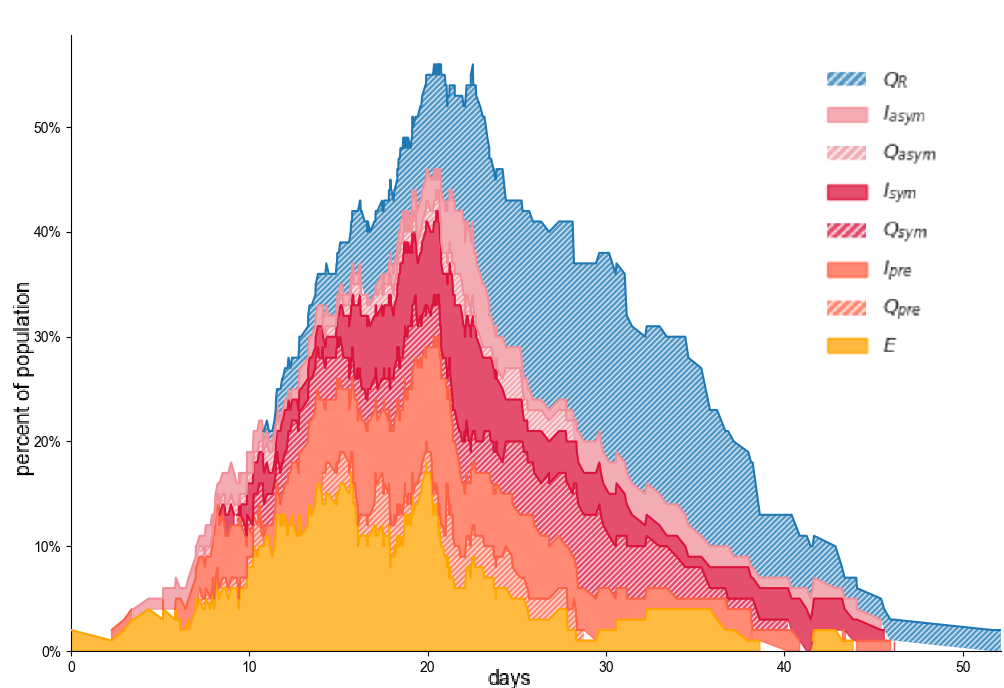
\includegraphics[width=\textwidth]{Figure3}
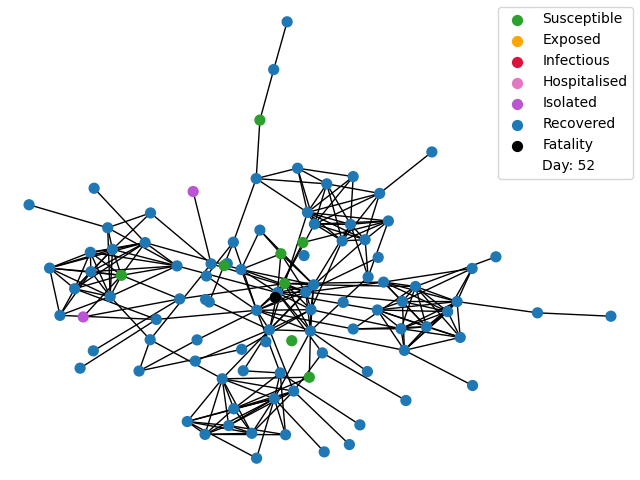
\includegraphics[width=\textwidth]{Figure3Net}
\caption{Benchmark Run with Unchanging Compliance at 50\% for regular twice weekly surveillance testing and testing if symptomatic with the resulting final network. 92 of the 100 agents received the infection}
\end{figure}

\newpage 

To simulate the childcare scenario the 100 agents are split into 5 groups of about 20 agents each with high connectivity inside the group and low connectivity between the groups. The edges in the network represent that particular agent's close contacts which the disease can spread easiest though. For the benchmark baseline, compliance for behaviour is set at levels of 0.5 and 1, to represent 50\% of agents and all agents complying. If agents are compliant, they will perform symptomatic test and regular interval surveillance tests when asked.\newline

The R0 (The disease basic replication rate) of 9.5 or 5.4 may be too high as it assumes children spread the disease at the same rate as the general population as well as all disease spread of children occurring in entirely in the childcare location which is probably not the case. Therefore two other R0 cases of 3 and 2 are used as they may more accurately capture a real world scenario where not all transmission is though the childcare setting. Additionally statistics are not currently available for an accurate R0 for young children to other young children, therefore the general population spread rates had to be relied upon. \newline

Two different runs of the benchmark model are run. Firstly a baseline of 50\% compliance, where each agent when generated has a 50\% chance to always or to never comply. The other is a baseline 100\% compliance, where each agent when generated has a 100\% chance to comply. 


\section{A Non-Strategic Behavioural Model}
The non-strategic model has two parts, a cost and benefit where benefits must outweigh costs to be compliant. 
The cost is fixed at a set value and given a value so that initially 50\% of agents will be compliant. 
A combination of global and local behavioural factors are be added to set an agents benefit, making an agent more compliant.
The global factor is the known positive cases in the network in the past 14 days. 
The local factor is the proportion of contact agents (those which share an edge) which are a fatality, hospitalised or in isolation. 
The benefit is taken away from the base cost and if the result is lower than a specified value, the agent will be compliant to that action, otherwise they are not.\newline

\begin{figure}[h!]
\centering
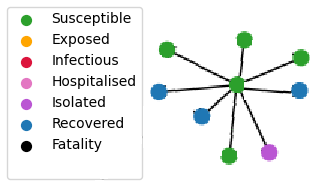
\includegraphics[width =150pt]{basicnet}
\caption{An example simplified network showing a single agent and their close contacts}
\end{figure}


With a case where 1\% of agents in the full network have reported a positive case in the last two weeks and one of the eight close contacts an agent has are in a high risk category, the calculated compliance would be one where the agent is compliant as the result is under 0.5

\[Compliance = 0.5 – (5 * 1/8) – (5*0.01) + 0.1 = -0.075\]


The agent would potentially become uncompliant if the close contact in isolation, recovered and left isolation as the new compliance equation would become one over 0.5 where the agent is no longer compliant.
\[Compliance = 0.5 – (0 * 1/8) – (5*0.01) + 0.1 = 0.55\]



Agents are given diversity in the non-strategic model. Initially a value is generated that is used in all compliance calculations for that agent. This either biases them to be more or less compliant, for example the base attitude for an agent might be 0.1; meaning the benefit would have to be 0.1 greater than that of a completely neutral agent for them to comply. This model is used for one case where the fixed cost is set at 0.5, this model is called the Non-Strategic Minimum 50\%.  In this model each day the compliance value for an agent is updated and changes. Factors that change the agents compliance a combination of the global known positive test cases recorded in the network within the last 14 days as well as the proportion of close contacts of an agent that are either symptomatic, a fatality, hospitalised or in isolation.\newline



\begin{tabular}{|c|c|}
\hline
Symptomatic Testing Rate Compliance & 50\% \\ \hline
Surveillance Testing Rate Compliance & 50\% \\ \hline
This agent’s base aptitude & uniformly distributed (-0.1,0.1) \\ 
&  set at 0.1 for this agent\\ \hline
Base Cost of Compliance & 0.5 \\ \hline
\end{tabular}
\newline


\newpage
\section{A Strategic Behavioural Model}
For the strategic model a strategic stag hunt game is played simmilar to the one explored in this paper~\cite{pacheco_santos_souza_2014}.  A curve is created to model a game theory dilemma on wherever or not each agent should comply, given they know the cost and reward for compliance and what every other agent will do. Depending on the benefit the agent sees for compliance, the likelihood of any one agent complying can vary from 0, to 60-99\% to 100\%. There is a level at which people will not contribute as they find the act pointless as they know near no agents will comply. This model is used in three cases which are discussed later and is designed like the non-strategic model to have a baseline of 50\% compliance. This will then grow based on the situation of each agent.\newline

\begin{tabular}{|c|c|}
\hline
Parameter & Value \\ \hline
Cost of Compliance & 1 \\ \hline
Overall benefit If action sucsessful & Depends on either a global or local situation\\ \hline
Minimum number of agents in  & 60\\ 
group complying to see benefit & \\\hline
Number of agents in group & 100\\ \hline
\end{tabular}
\newline

The value benefit  is assigned can be grouped into 3 categories. Strategic Community Size is where the benefit to compliance is based on the number of close contacts the agent has. This is a case where the curve is different for each agent but unchanging over time. Strategic Local State is where the benefit to compliance is based on the number of close contacts that are either in a state of symptomatic, a fatality, hospitalised or in isolation. This is a case where the curve is different for each agent and unchanging over time. Strategic Global State is where the benefit to compliance is based on the number of agents in the network that are either in a state of symptomatic, a fatality, hospitalised or in isolation. This is a case where the curve is the same for each agent but changes over time. \newline

\begin{tabular}{|c|c|c|}
\hline
Model & Benefit Curve  & Benefit Curve\\ 
&is different for each agent &changes over time \\\hline
Strategic Community Size & Yes & No \\ \hline
Strategic Local State & Yes &Yes\\ \hline
Strategic Global State & No &Yes\\ \hline
\end{tabular}
\newline


\begin{figure}[h!]
\centering
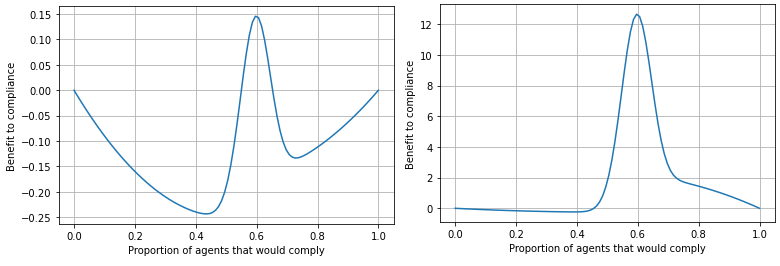
\includegraphics[width=12cm]{strat}
\caption{Comparison of two extreme examples of compliance curves with a very low (50) and very high (1000) benefit to compliance, the game is run with a cost of 1, 100 agents and 60 must be compliant to see a benefit}
\end{figure}

In figure 5 the chart on the left has two points of compliance 0 and 0.65, This is because if the agent was between 0 and 0.55 they would see compliance as not worth it as their overall benefit to compliance in the system is negative and move towards a compliance of 0. If the agent was between .55 and 0.65 they would move towards 0.65 as the benefit to compliance is still positive for more agents to comply. Finally if the agent was between 0.65 and 1 they would move towards 0.65 as the benefit to compliance is negative, so the additional compliance is not rewarded. This creates a system with two absorbing states 0 with a weight of 0.65 and 0.65 with a weight of 0.35, in this case the state of 0 is dominant, so this agent would comply 0\% of the time. \newline\newline
On the other hand, the chart on the right has two points of compliance at 0 and 1. If an agent was between 0 and 0.45 they would see compliance as not worth it as their overall benefit to compliance in the system is negative and move towards a compliance of 0. If the agent was between 0.45 and 1 , benefit is positive for more agents to comply. This creates a system also with two absorbing states, 0 with a weight of 0.45 and 1 with a weight of 0.55, in this case the state of 1 is dominant, thus the agent would comply 100\% of the time.


\section{Results}

To evaluate the result of the model, those of the baseline, non-strategic and strategic we look at two key parameters, the percentage of agents that contracted the disease and the number of days that elapsed until zero agents were infectious. In this model two states of compliance are considered, If an agent is compliant they will perform semi-weekly surveillance testing in addition to testing whenever they develop a symptomatic case of the disease, If they are not compliant they will do neither of these actions. All agents will always isolate immediately after receiving a positive test result. The results of these models are computed from 50 separate runs for each, model/R0 combination. \newline

\newpage

\begin{figure}[h!]
\centering
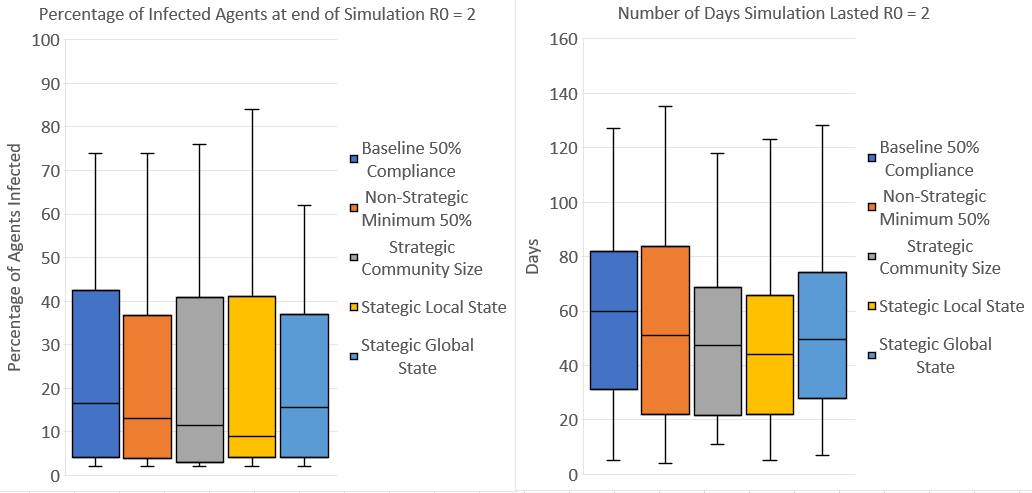
\includegraphics[width=\textwidth]{5}
\caption{Test Results over R0 of 2}
\end{figure}

\begin{figure}[h!]
\centering
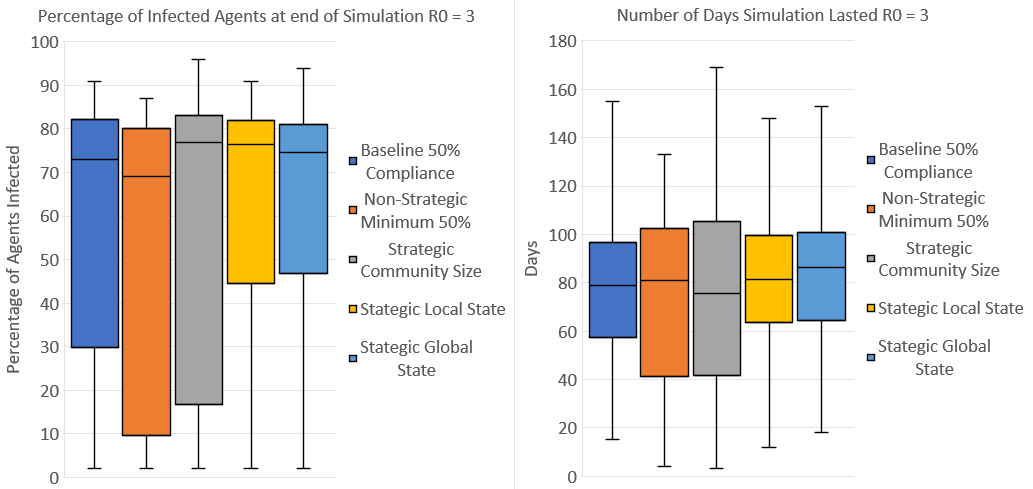
\includegraphics[width=\textwidth]{4}
\caption{Test Results over R0 of 3}
\end{figure}

\newpage

\begin{figure}[h!]
\centering
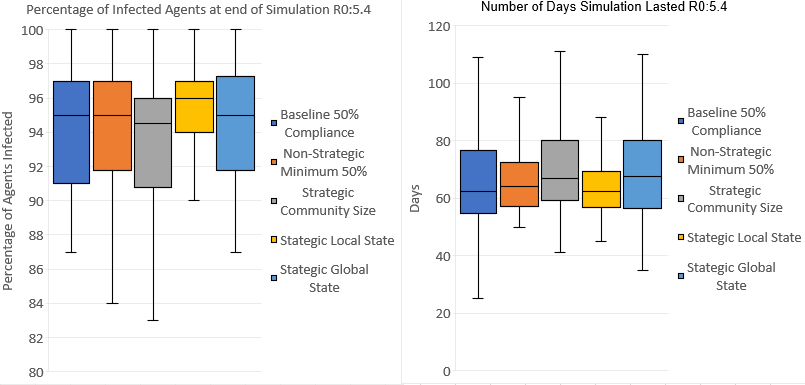
\includegraphics[width=\textwidth]{3}
\caption{Test Results over R0 of 5.4}
\end{figure}

\begin{figure}[h!]
\centering
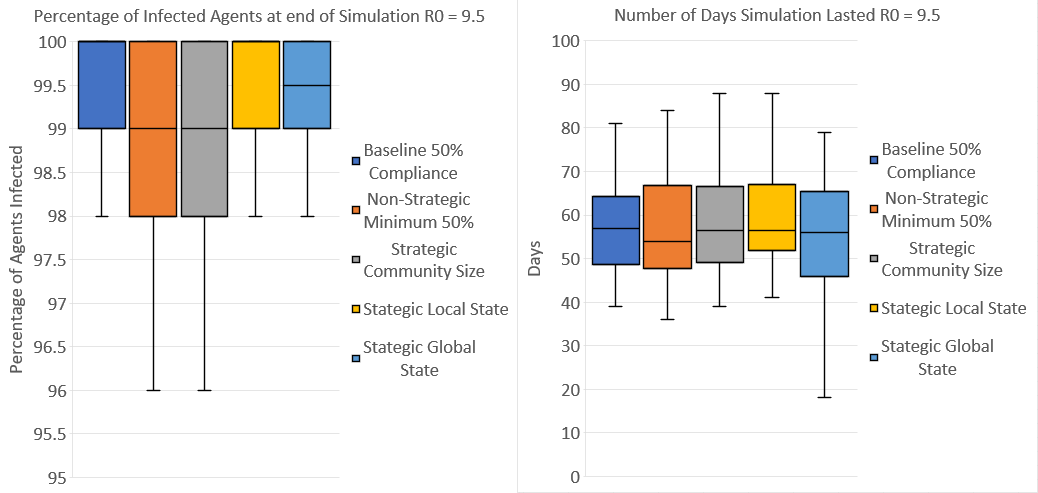
\includegraphics[width=\textwidth]{2}
\caption{Test Results over R0 of 9.5}
\end{figure}
\newpage

\begin{figure}[h!]
\centering
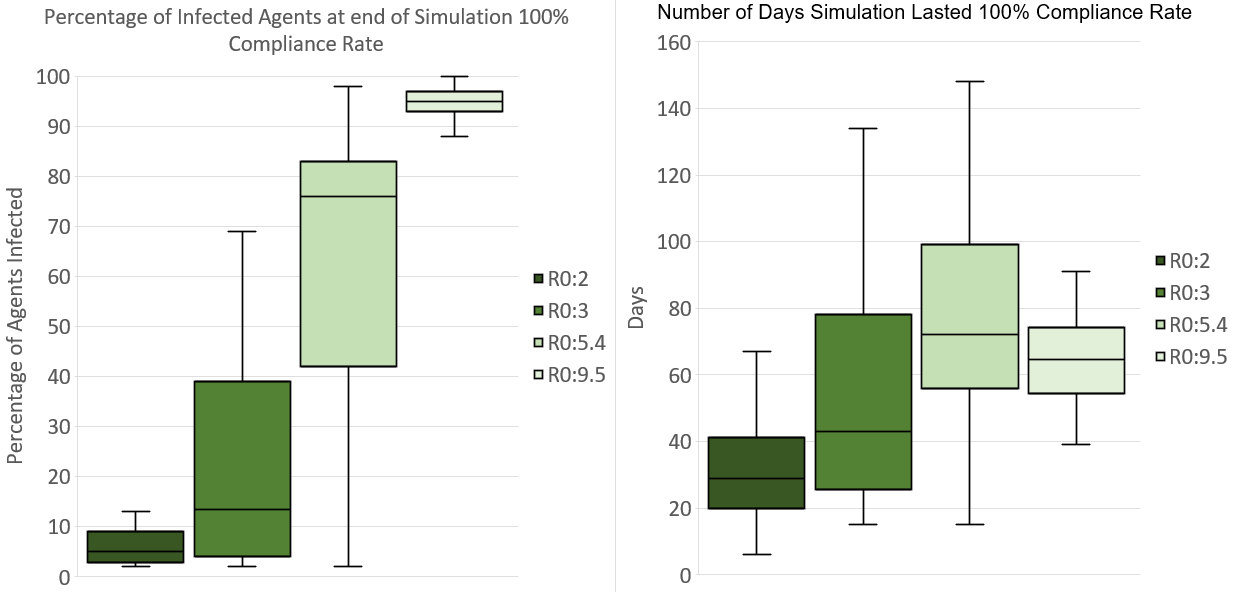
\includegraphics[width=\textwidth]{6}
\caption{Test Results over all R0 values at 100\% Compliance}
\end{figure}

\begin{figure}[h!]
\centering
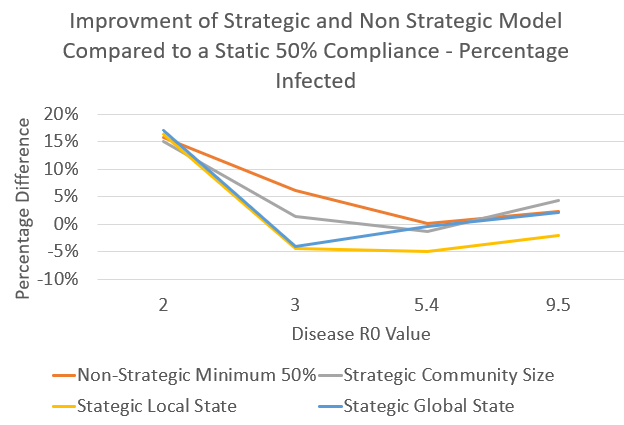
\includegraphics[width=\textwidth]{1}
\caption{Test Results Comparing the Results of R0 values}
\end{figure}
\newpage


\section{Discussion}

\subsection{Analysis of total infection size}

Each of the models was run over 4 different R0 virus base reproduction rates. The higher the Disease R0 the more infectious it is. The Improvement the models had over the base 50\% compliance baseline saw an improvement from -5\% at the high R0 values to 17\% at the low R0 values. The non-strategic model was found to be the most effective in reducing the number of infected agents throughout the R0 values of 2 (16\%), 3 (6\%) and 5.4 (0\%) but by 9.5, the strategic community size model was found to be more effective with a 4\% reduction of disease spread (figure 11). This could be a result of the non-strategic model taking into account both the global spread of the disease in the network as well as the current compartment / state of close contacts impacting compliance. In the case of an extremely high R0 values the strategic community size model was most effective.  This model only considers the number of close contacts an agent has when deciding if they are compliant or not. This could be the case as it forces those most central agents to be compliant. Therefore, they are not able to spread the disease far across the network, forcing it to stay more localised where it has the opportunity to die out before it becomes an epidemic in the network.\newline 

The models were likely more effective on the lower R0 values as the agents have more time to choose to be compliant. As the disease spreads slower though the system, there is more time for compliant agents to go through a run of surveillance testing and potentially isolate before they have infected many other individuals. With extremely high R0 numbers it is observed that the non-strategic and strategic behavioural model have little effect on the total number infected (i.e. all having $< 5$\% improvement). 


\subsection{Analysis of Epidemic Duration}

Regarding the days the simulation took before disease spread stopped, it was found that the strategic models particularly at the lower R0 values of 2 and 3 saw significant improvement over the 50\% baseline tests. This is interesting as while similar percentages of agents were infected, the time it took for the disease to die out was less, suggesting the disease spread through the network faster but ultimately had about the same proportion of agents who ended up getting the disease.\newline 

Notably the case of Strategic Local State where agents use the number of agents around them who are in a high risk state to decide if they are compliant fared the worst at a disease R0 value of 9.5 having a 2\% increase in infected agents and it taking 6\% longer for the disease to stop spreading (figure 11). This would suggest that agents who based decisions about if to test based solely on how their close contacts are faring is not a good approach at reducing the spread of disease and more global measures or measures that rely on how central a person is in their network of close contacts are more effective. \newline 

There are a few areas in which future work could be conducted, some areas would include; Modifying the model to allow for vaccinated agents, as this would more accurately mirror the real world situation we now have with a vaccinated population. Creating a network which assigns the agents ages which would have an impact on various parts of the model such as disease test false negative rates, hospitalisation and fatality rates as well as potentially R0 values for the specific agents. This would create a more accurate simulation as the false negative rate for rapid tests varies significantly with age and for the purposes of this paper the disease and testing parameters for infants / young children were applied to everyone. Furthermore, the models could be expanded by forcing all or sections of the network to enter quarantine for a period of time under certain conditions, to control spread in the network. This would be able to simulate the day-care closing for a period of time due to a very high spread of the disease.

Concludin thoughs .....

\newpage

\bibliography{bibliography}{}
\bibliographystyle{plain}

\newpage
\appendix

\section{Appendix}
The code for the models can be found at \url{https://github.com/robertmxmx/seirsplus-dynamic-agents}.
The format for this paper is based on a journal submission for PLOS Computational Biology.

\end{document}


\end{document}

